\begin{figure}[H]
    \centering
    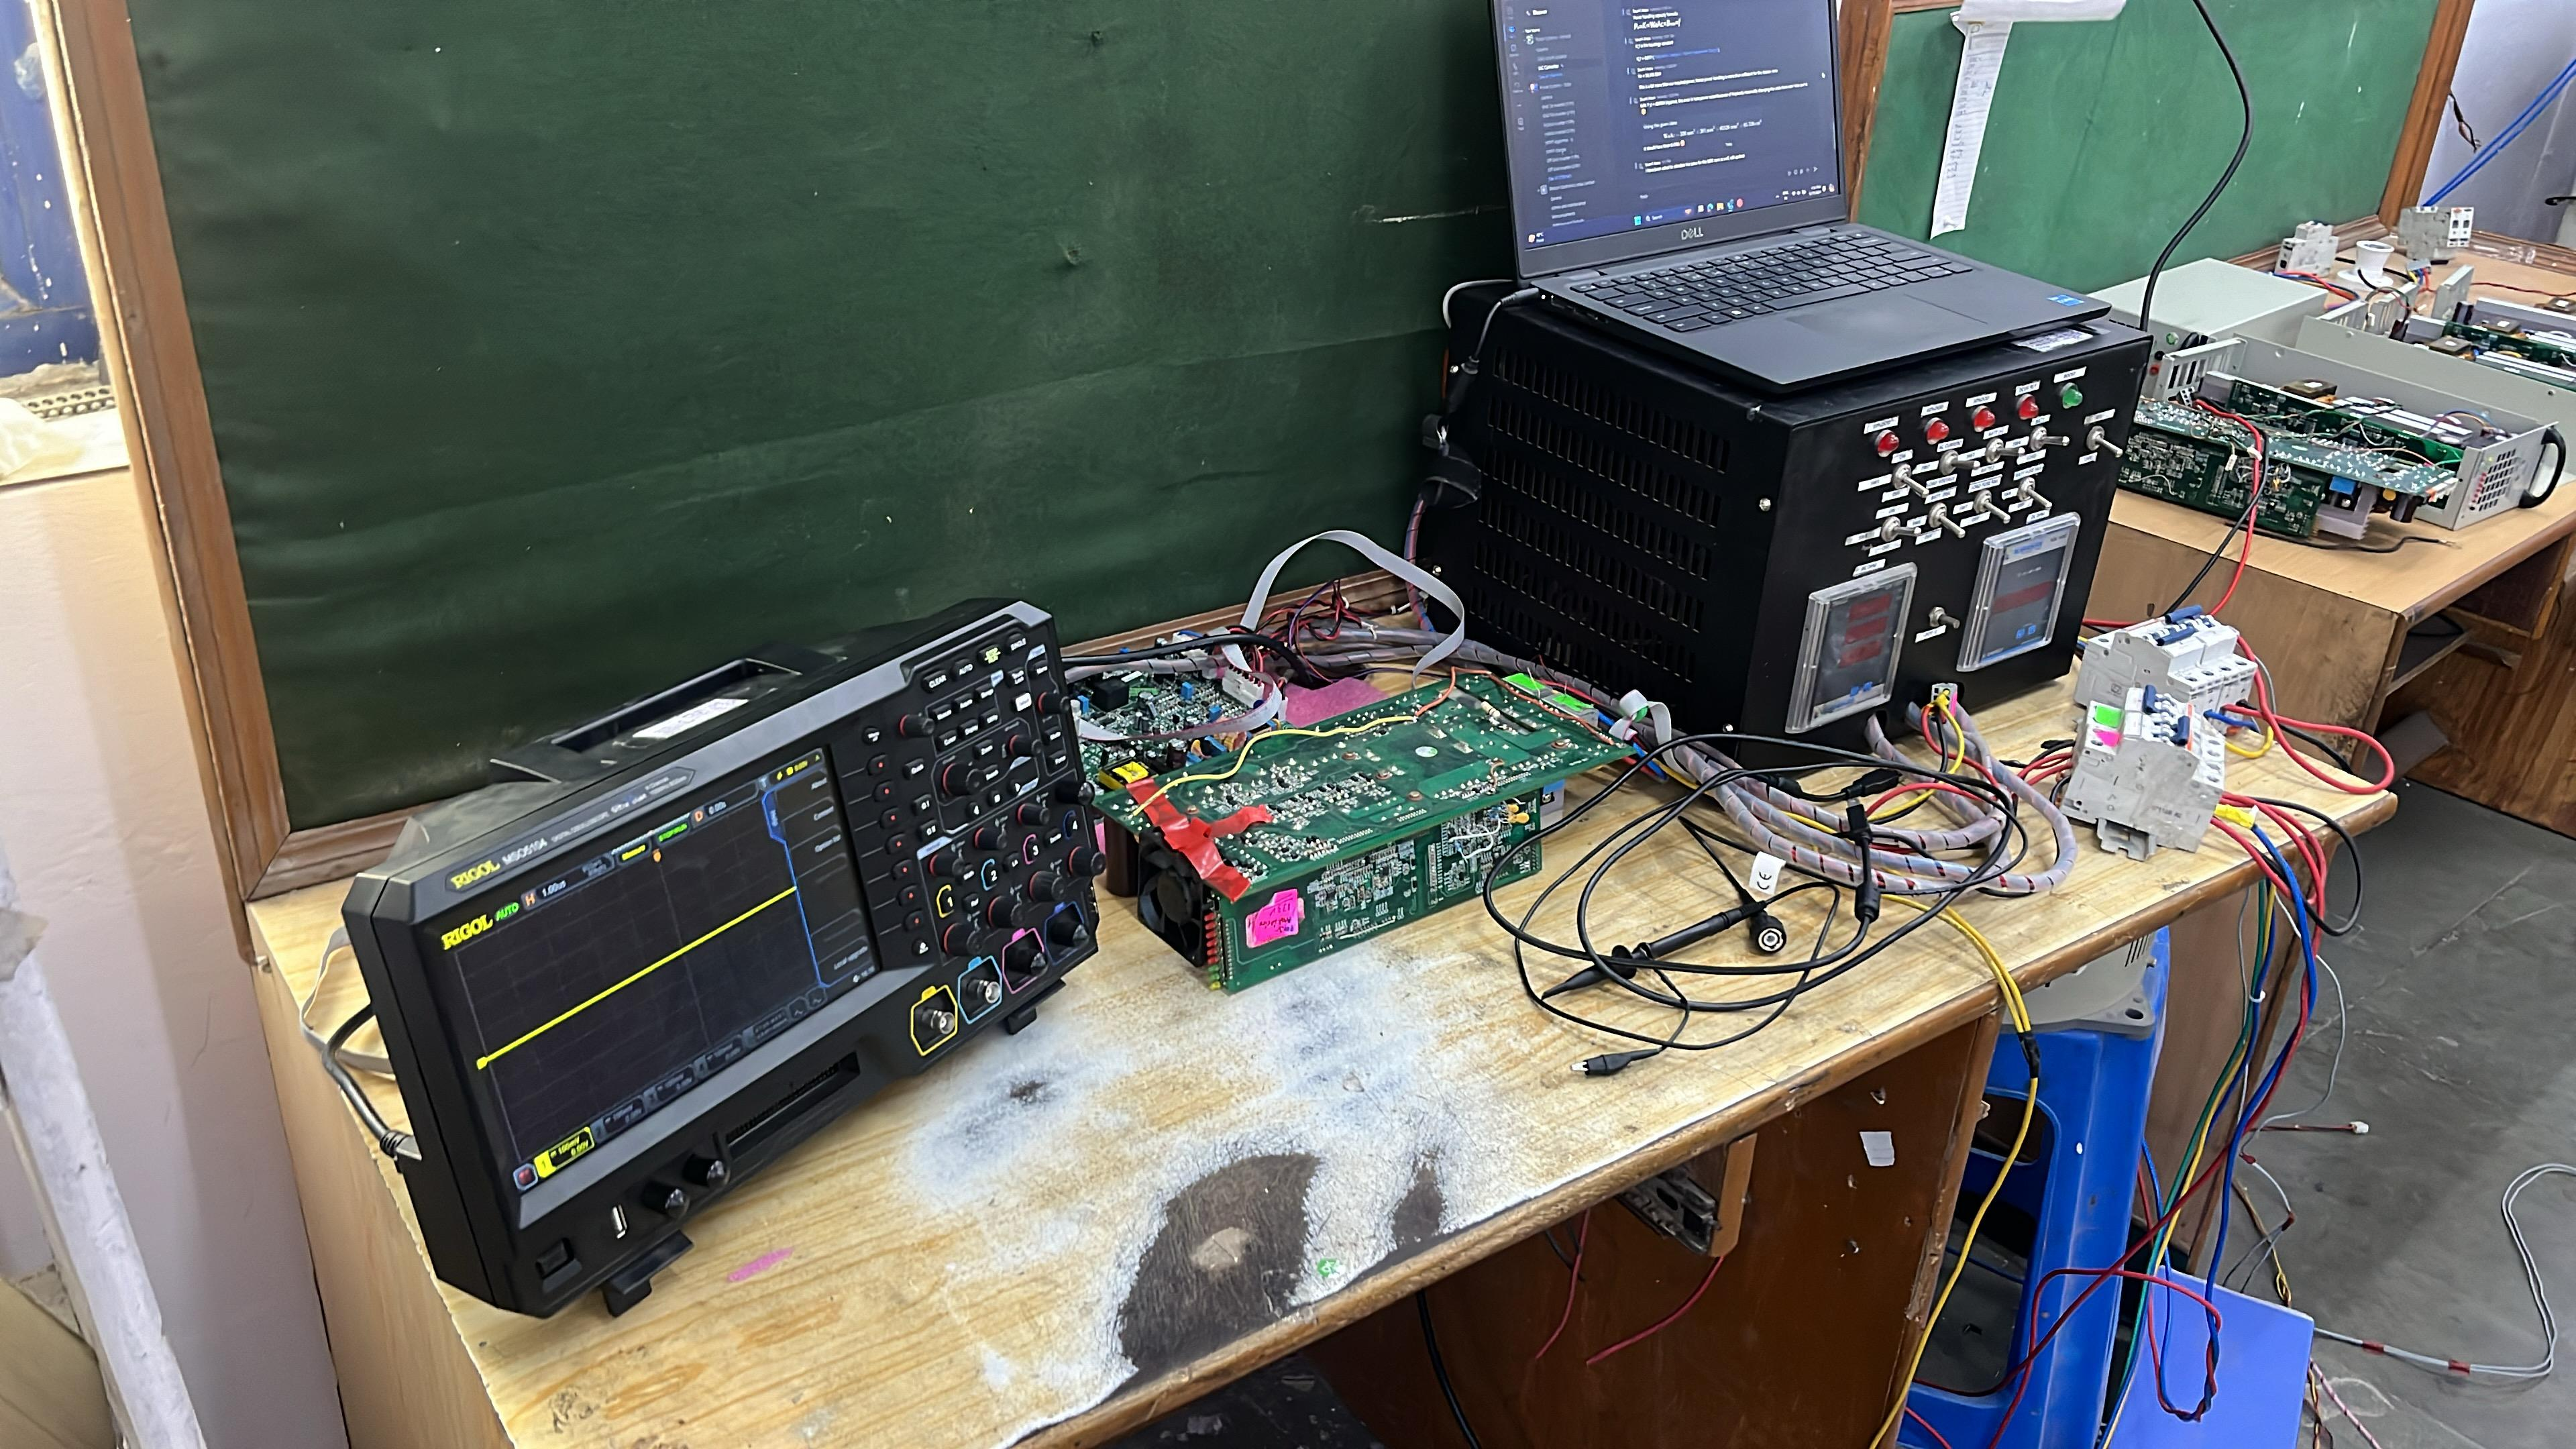
\includegraphics[width=0.6\textwidth]{overall_setup.jpg}
    \caption{Hardware Testing Setup}
    \label{fig:overall_setup}
\end{figure}

\begin{figure}[H]
    \centering
    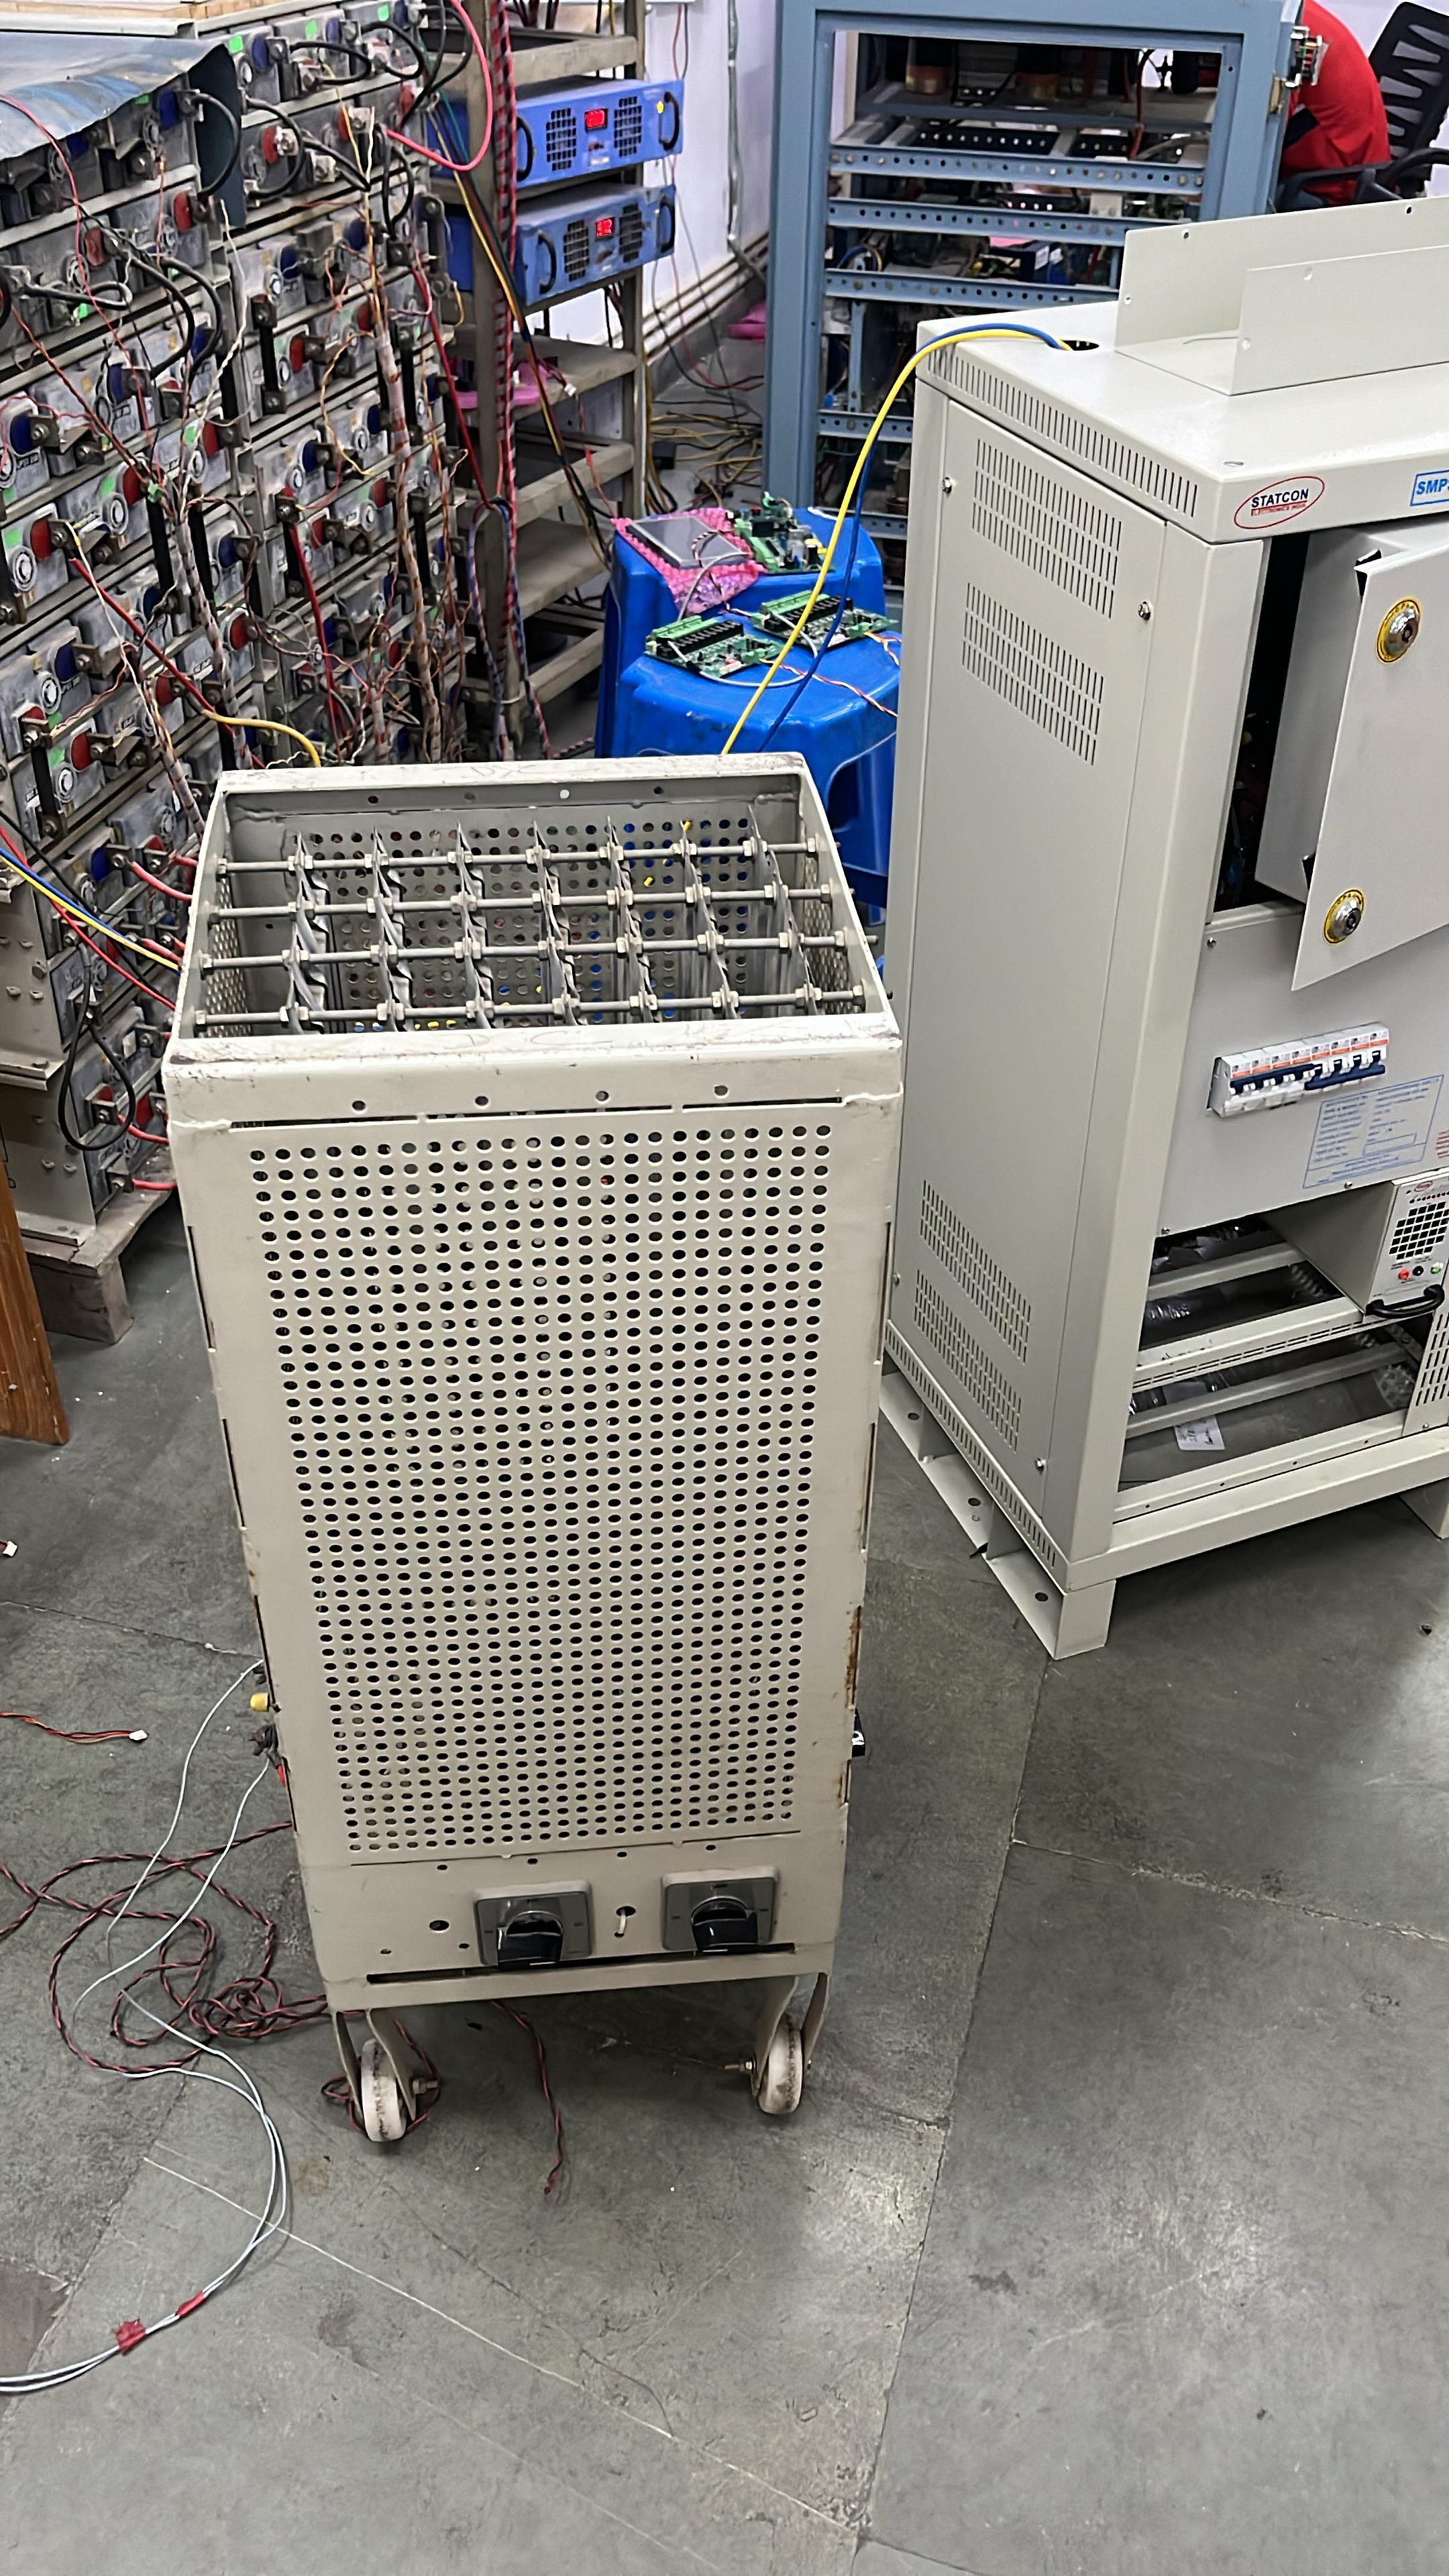
\includegraphics[width=0.3\textwidth]{load.jpg}
    \caption{The load that we made for testing}
    \label{fig:load}
\end{figure}

\begin{figure}[H]
    \centering
    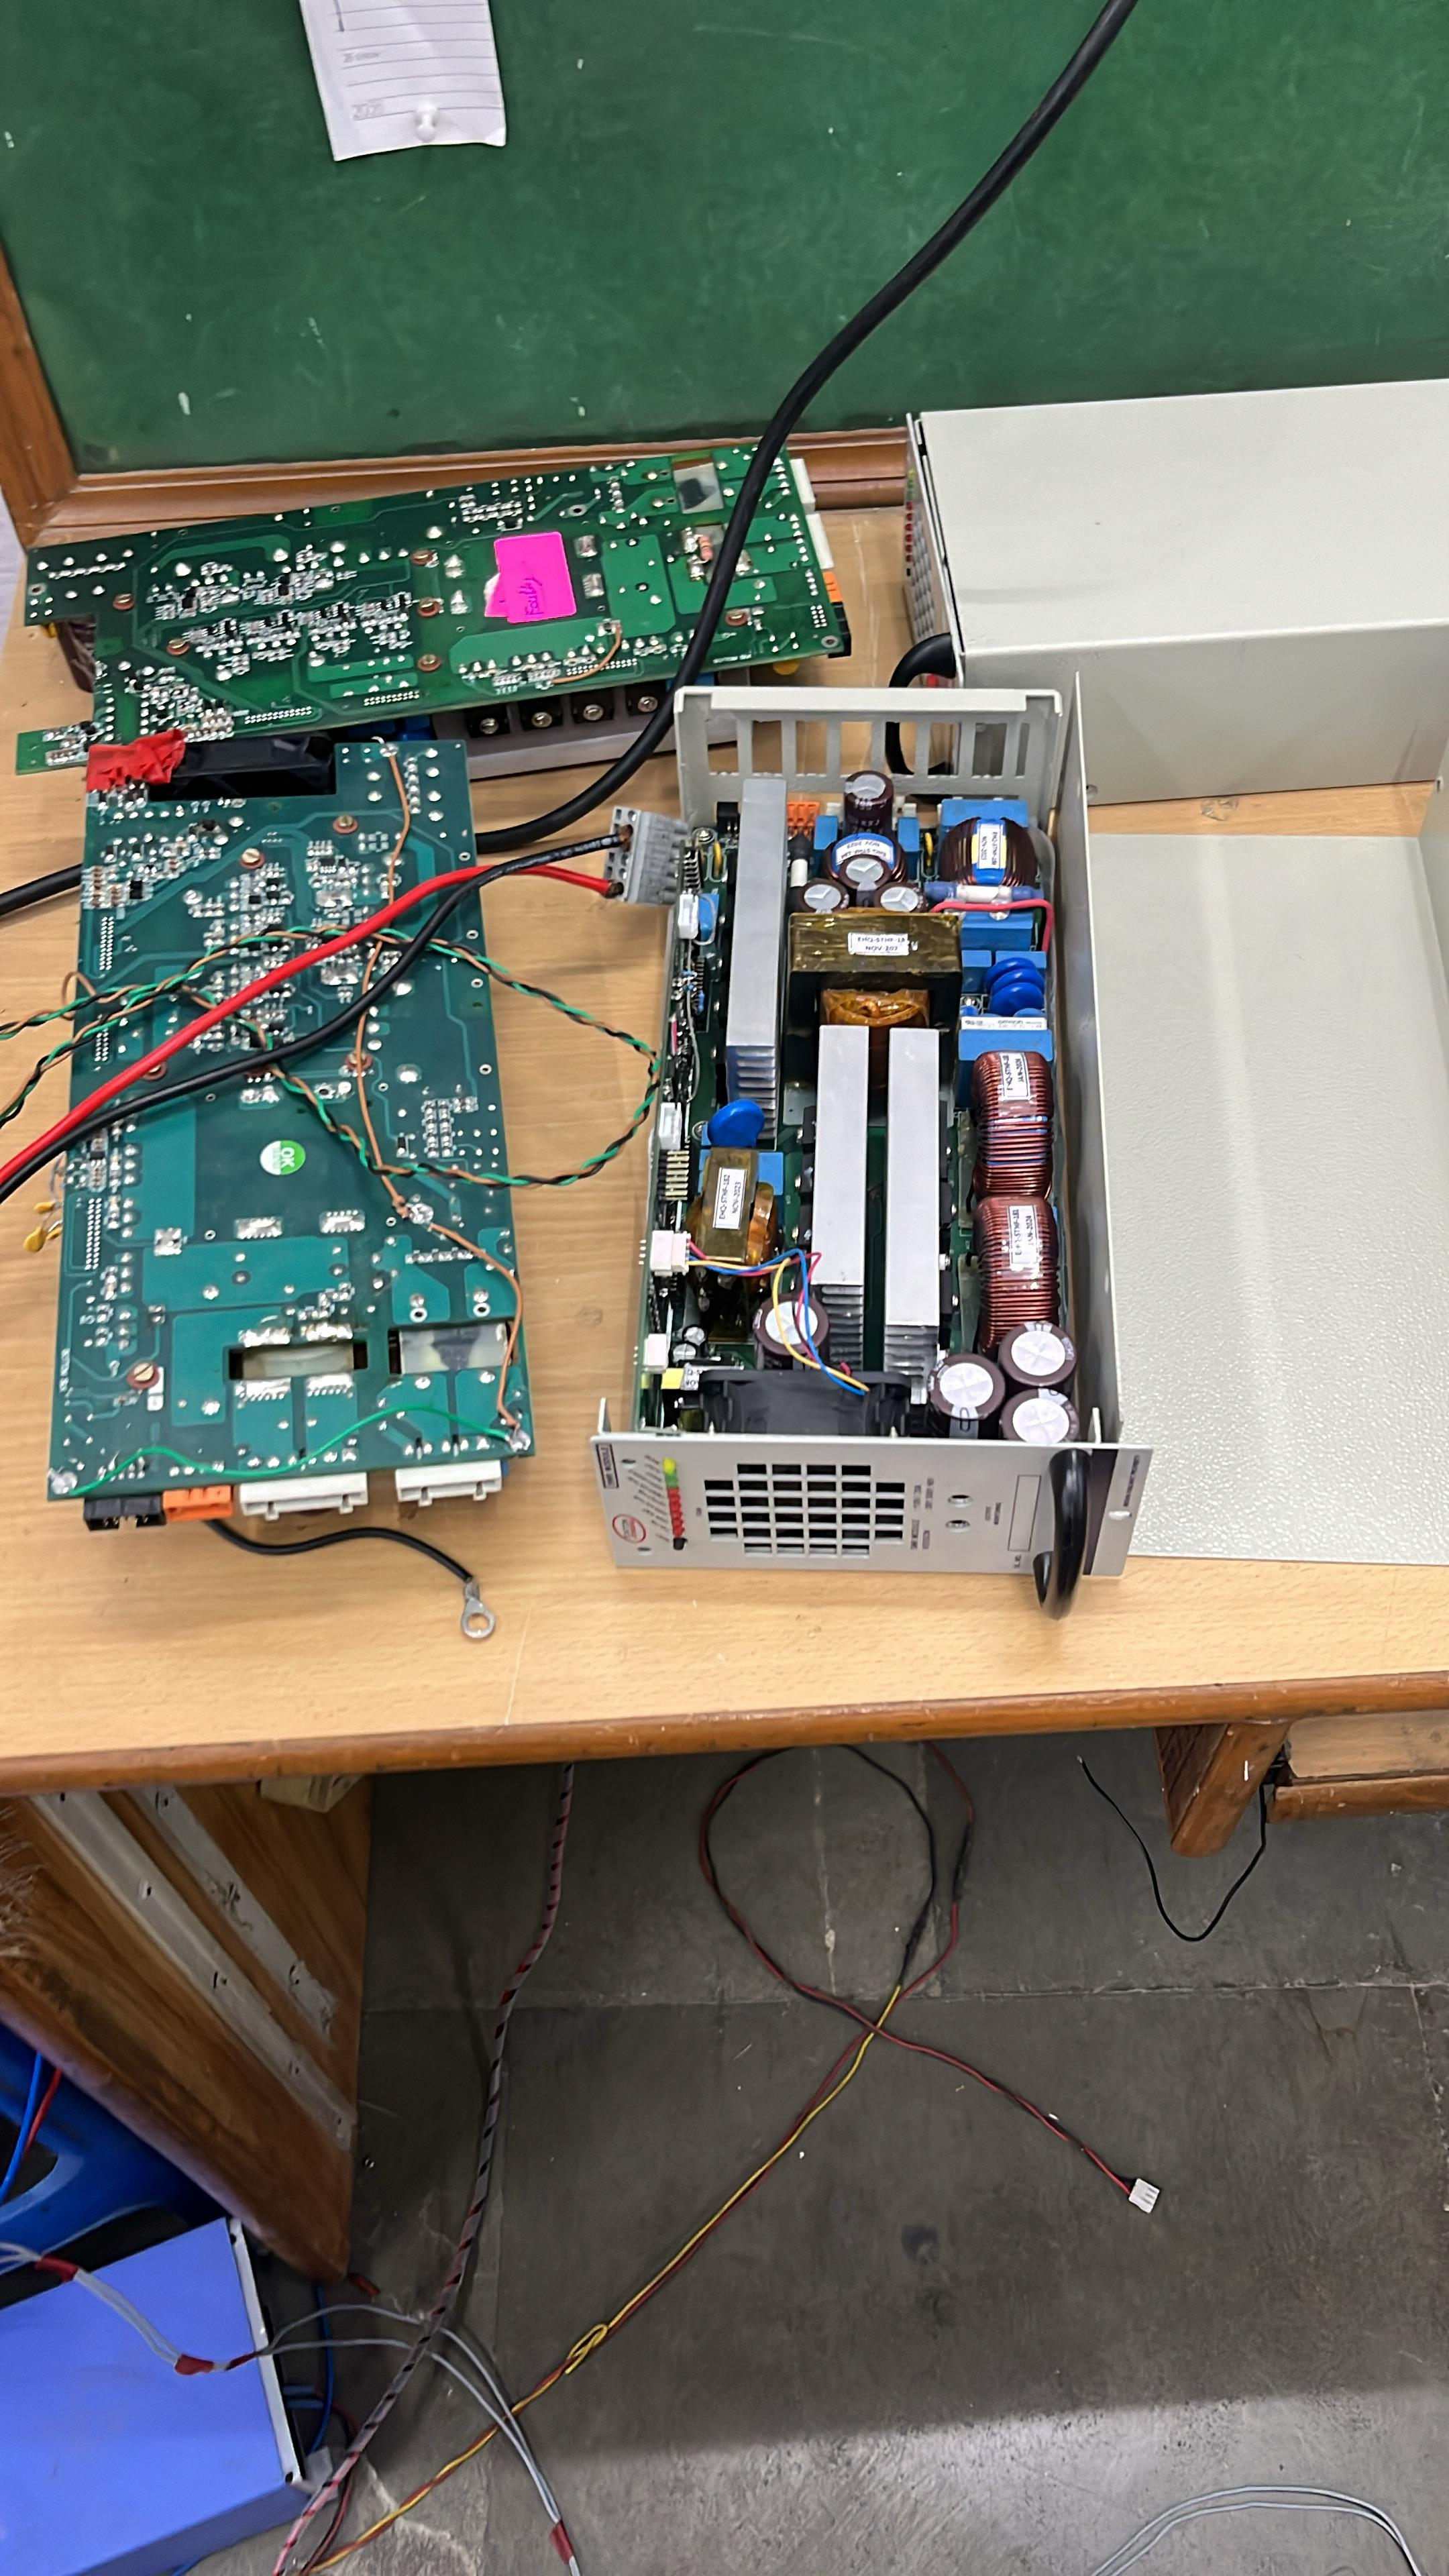
\includegraphics[width=0.3\textwidth]{top-bottom.jpg}
    \caption{The assembled circuit}
    \label{fig:top-bottom}
\end{figure}

\begin{figure}[H]
    \centering
    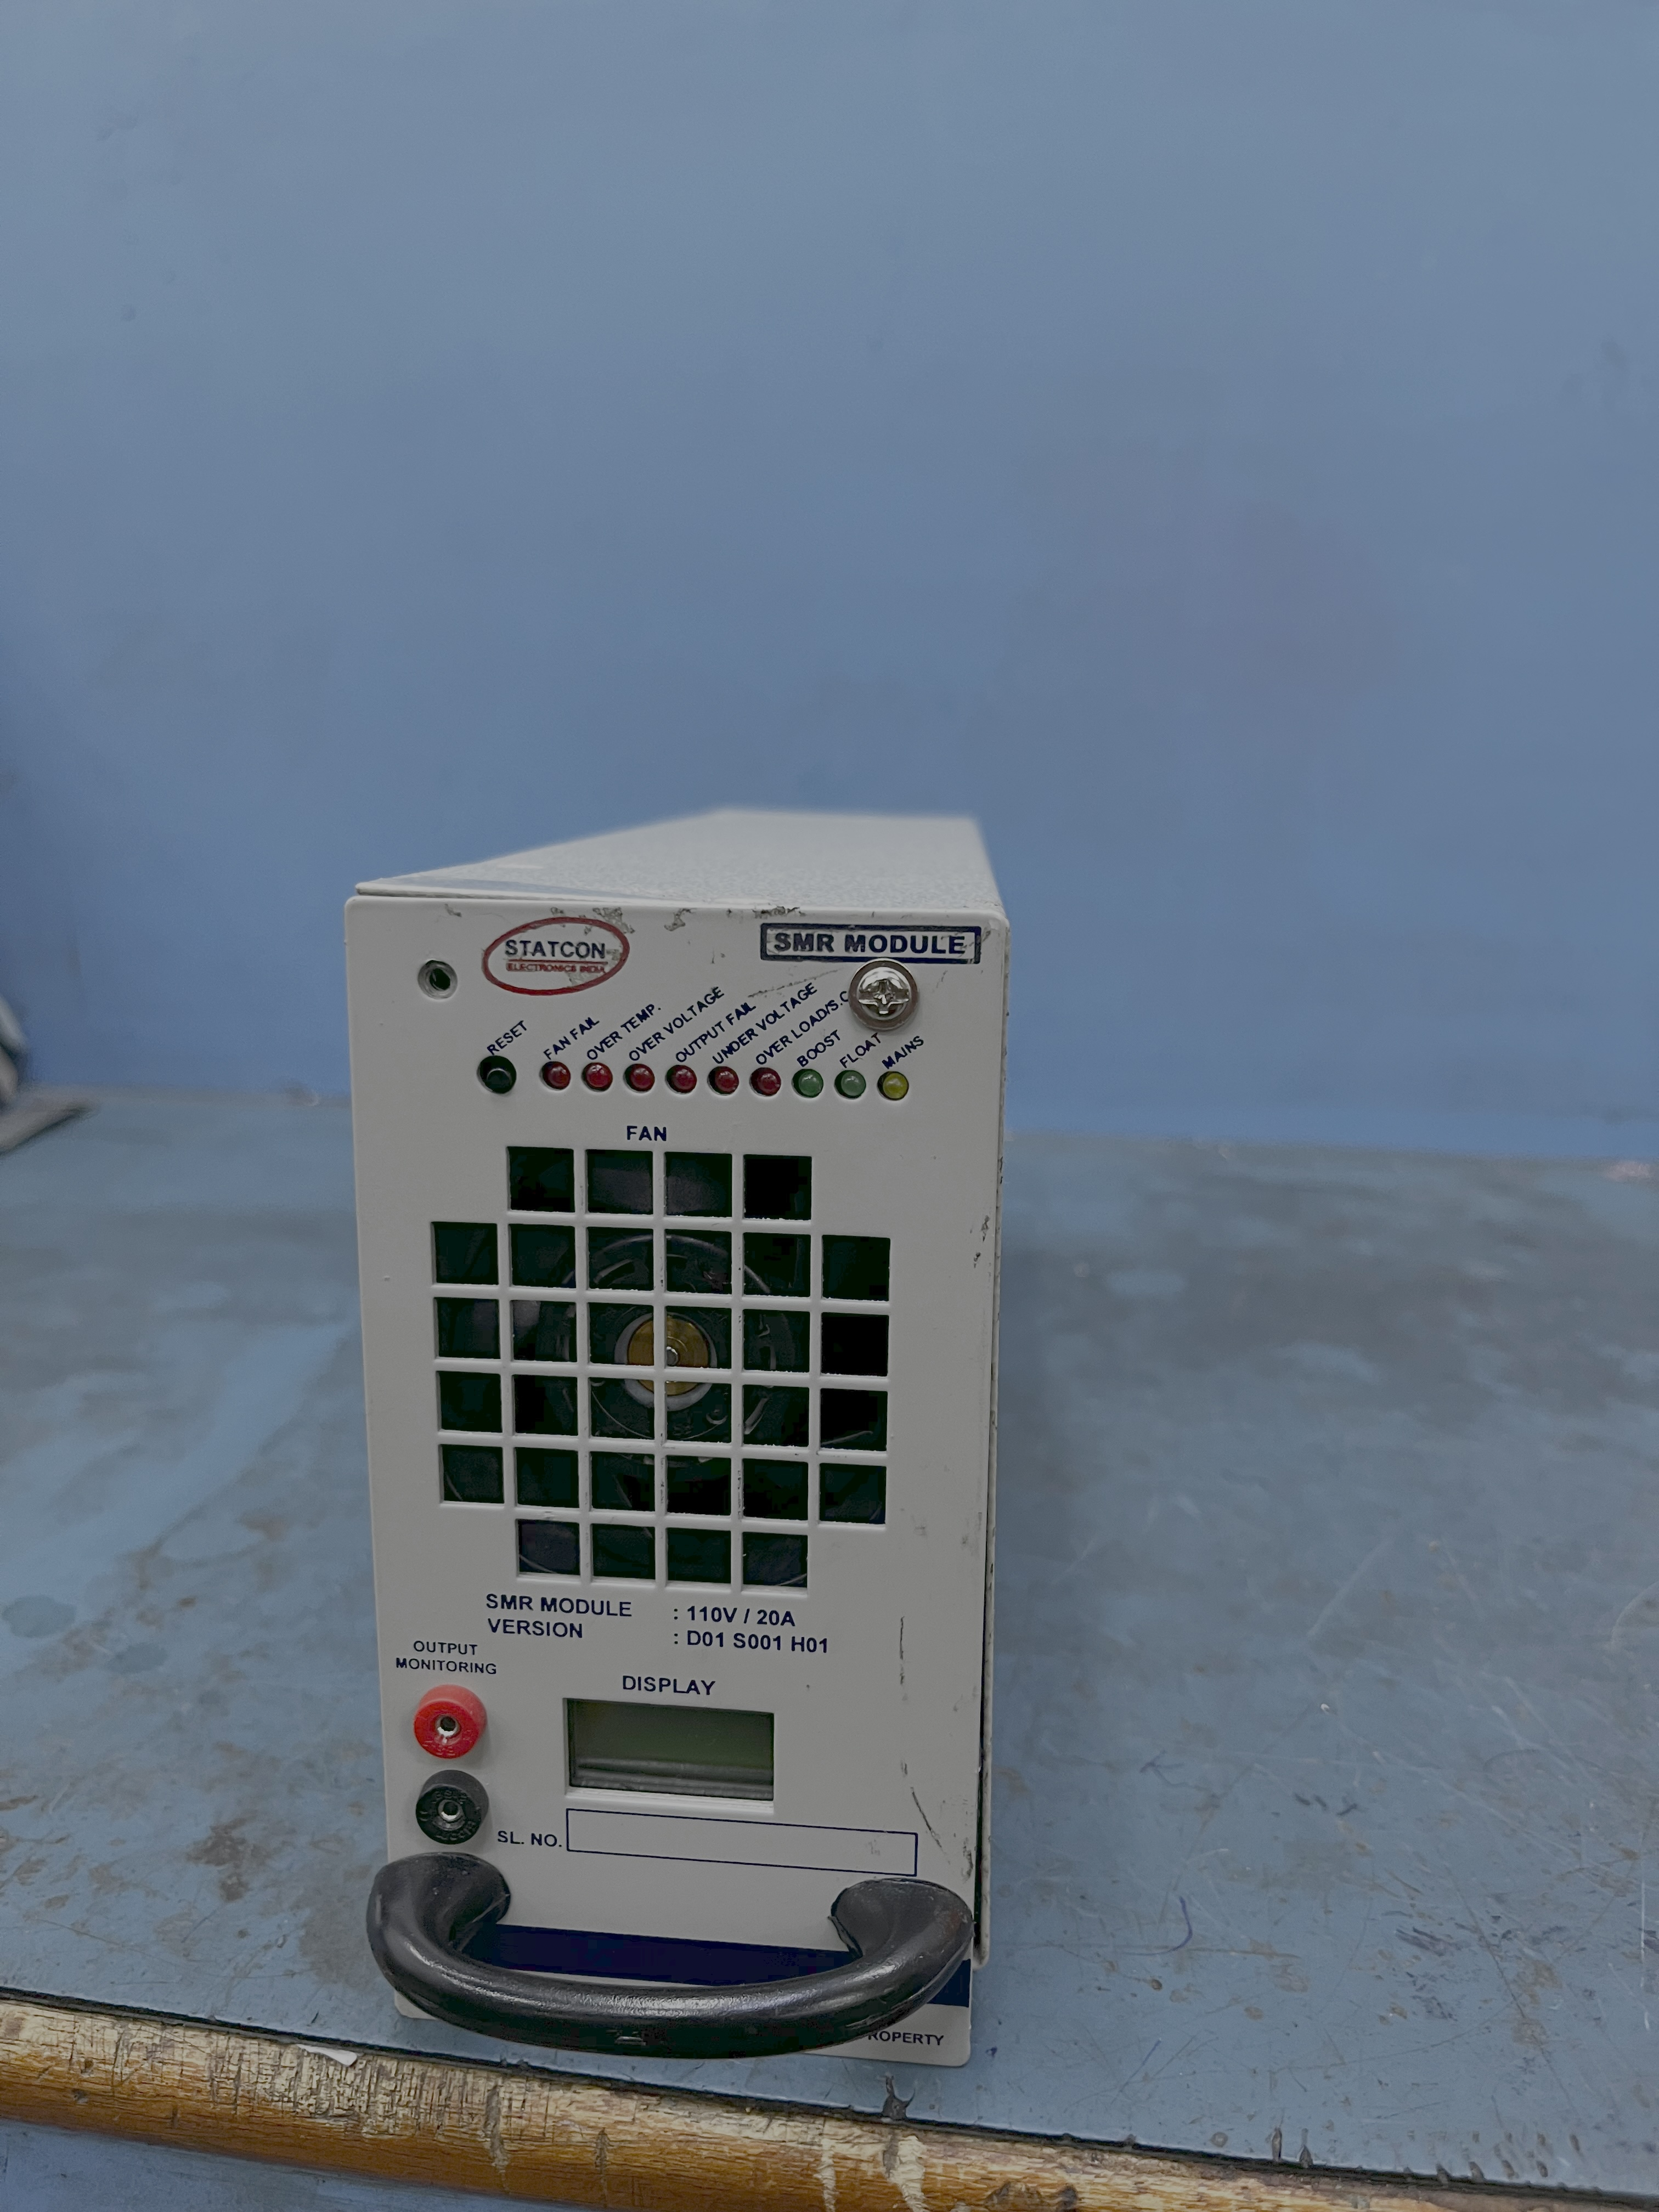
\includegraphics[width=0.3\textwidth]{complete-assembly.jpg}
    \caption{Completely assembled circuit}
    \label{fig:complete-assembly}
\end{figure}

During the hardware testing and debugging of the circuit, I faced many issues to resolve, some of which were:
\begin{itemize}
    \item \textbf{Issue in the voltage feedback signal}: The output voltage was having fluctuations, which we found out was because of noise in the feedback signal of the voltage produced.\\
    To overcome this issue, we experimented with values values of voltage divider resistors, and capacitors so as to minimise the noise in that signal and somewhat stabilize the output.
    \item \textbf{Issue with boost of the converter}: The converter did boot up properly (going from 90V at startup to 120V, which is the voltage at the resonant frequency as well), but if wouldn't go past that (it should go till 150V). Though this issue was observed only in some converters and rest did not have this issue, the cause of this issue needed to be found out toe nsure reliablility across products when it's finally put into production.\\
    The issue was identified as noise in the connector which carries the "Set output DC Voltage" signal (basically the DC output voltage which it must make), which is sent with the DSA Board (another board which is connected to the motherboard which communicates with the battery etc and conveys the information as set output voltage, maximum current flow etc. to the LLC Converter control board).\\
    The issue was resolved by passing the connector through a ferrite bead (Figure \ref*{fig:ferrite-bead}). This acts a common-mode choke and helps filter out the common-mode noise, allowing only differential signals to pass through. It also helps in controlling the impedence ensuring signal integrity over the length of the connector.
    \begin{figure}[H]
        \centering
        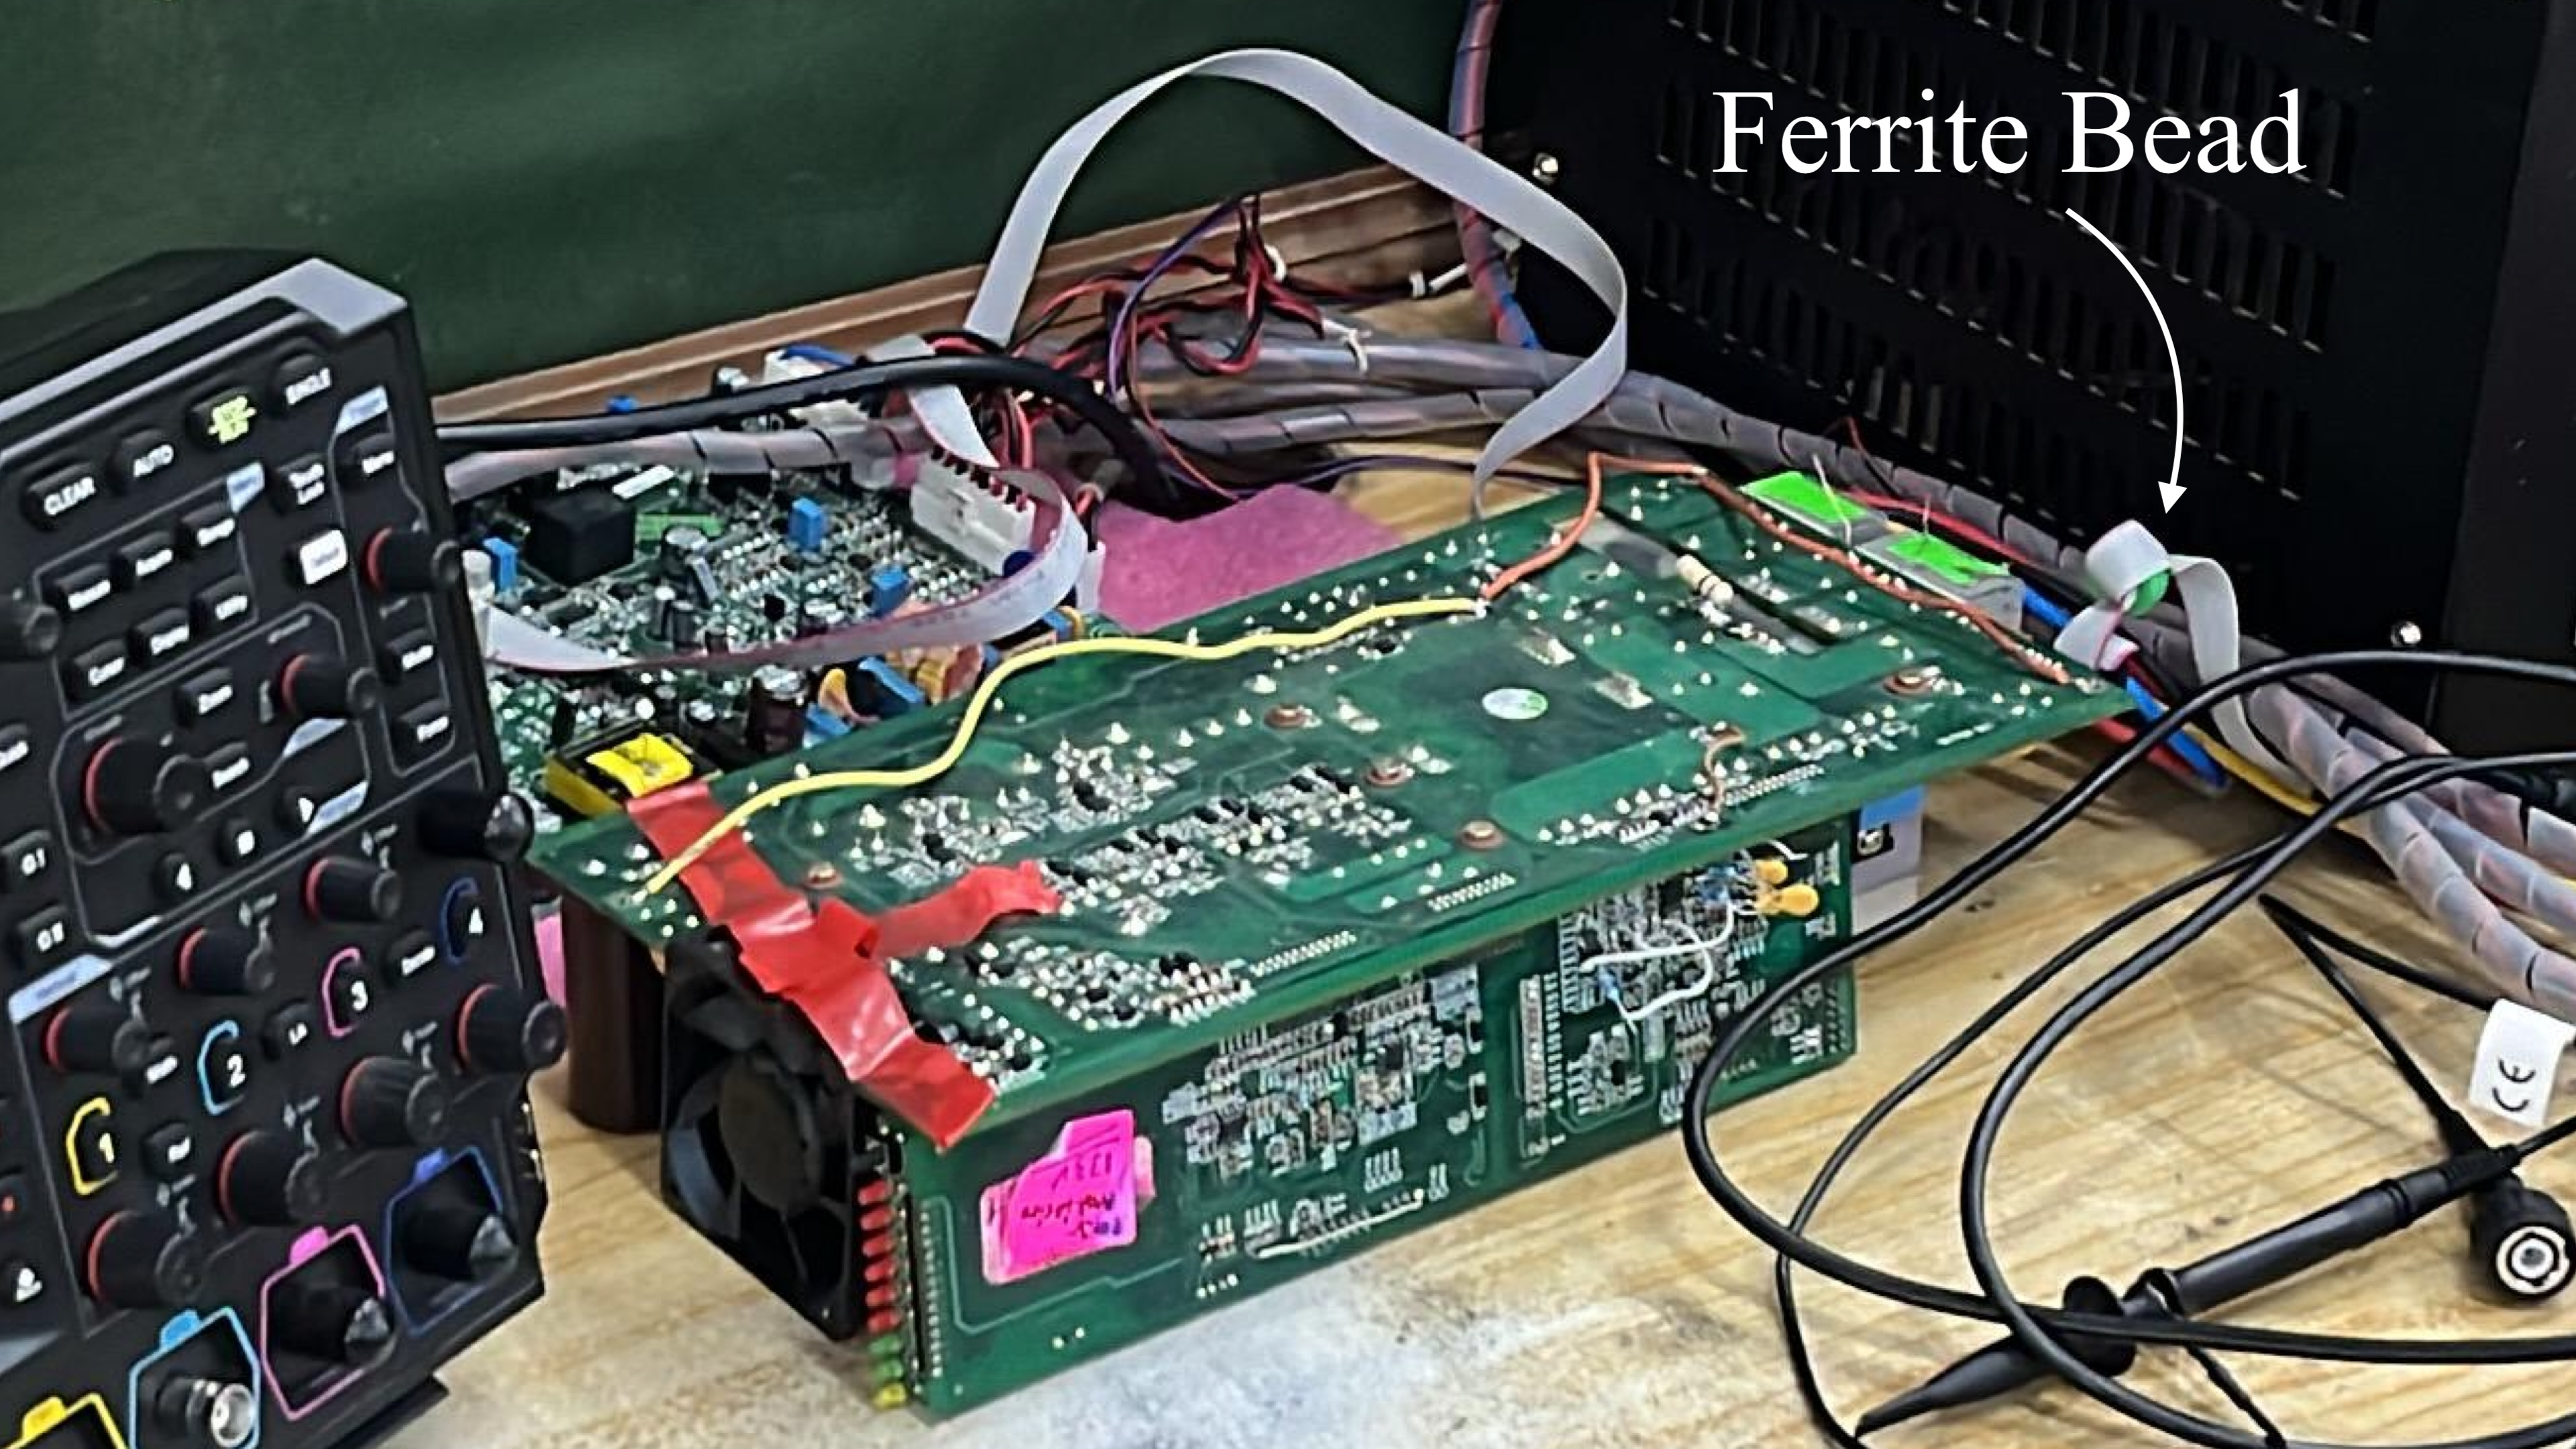
\includegraphics[width=0.6\textwidth]{ferrite_bead.jpg}
        \caption{Ferrite Bead (See Arrow)}
        \label{fig:ferrite-bead}
    \end{figure}
    \item \textbf{Load Sharing}: The ultimate aim of our converter is that multiple converters will be hooked up in parallel connected to a single DSA board (which will let know each one of them about the desired voltage etc.).\\
    When we did that, the issue was that, say we have a load that requires 10A and we have 2 converters connected, so ideally both should output 5A for equal load sharing but the issue was that it booted up perfectly fine but as soon as there was a change in load, say the load increased to 20A, now each should output 10A, but there were oscillations in this, as well as the output voltage each one was producing. The oscillations in current were as large as 2A (like at some moment, one is giving 5A and other is giving 15A, and after some moments, the first one is giving 15A, while the second one is giving 5A).\\
    By my detailed analysis of the schematic, we figured out that this issue was because of the place at where we were measuring the output voltage and current of each converter for feedback and active control. There were separate GNDs for the feedback signal (Signal GND) and the output voltage (PWR GND) and because of presence of fuse and a choke at the output (to reduce the output voltage ripple), there was a difference in the potentials of both these GND (although in mV, but enough to cause oscillations in the output voltage, and hence output current).\\
    We resolved this issue for now by adding an offset for the voltage drop (by multiplying the current flowing by the resistance, this is a generalised value for each converter), but in the next version of the PCB, we will add a summing op-amp into the feedback signal to account for this difference in the potentials, which would eliminate the need for adding a offset.
\end{itemize}